\documentclass{article}
\usepackage{graphicx} % Required for inserting images
\usepackage[margin=2cm]{geometry}
\input{setup}
\usepackage{polski}
\title{Wyznaczanie stanów w jednoelektronowych kropkach kwantowych}
\author{Marta Wleklińska}
\date{\today}

\begin{document}

\maketitle



\section{Wstęp}
W poniższym ćwiczeniu rozpatrywana była kropka kwantowa, w której funkcję falową elektronu $\psi(\mathbf{r})$ chcieliśmy przedstawić w postaci kombinacji liniowej o współczynnikach $c_i$ funkcji bazowych $\varphi_i(\mathbf{r})$ (gaussowska)
\begin{equation}
    \psi(\mathbf{r}) = \sum_{i=1}^Nc_i\varphi_i(\mathbf{r}).
\end{equation}
Układ był rozpatrywany w dwóch wymiarach, wobec tego funkcje bazowe przyjmowały postać
\begin{equation}
    \varphi_k (x, y) = A_x A_y \exp\left[-B_x\left(x - x_k\right)^2 - B_y \left(y-y_k  \right) ^2 \right],
\end{equation}
przy czym $A_x, A_y, B_x, B_y$ są stałymi charakteryzującymi szerokość gaussianów.\\
\\
Problem sprowadza się do rozwiązania równania Schr{\"o}dingera
\begin{equation}
\hat{\mathbf{H}} \psi(\mathbf{r}) = E \psi(\mathbf{r}),
\end{equation}
gdzie hamiltonian składa się z operatora kinetycznego i potencjalnego. 
Użycie funkcji gaussowskich jako bazy umożliwia obliczenia analityczne dla macierzy Hamiltonianu $\mathbf{H}$ oraz macierzy przekrywania $\mathbf{S}$:
\begin{equation}
S_{ij} = \int_{\mathbb{R}} \varphi_i(\mathbf{r}) \varphi_j(\mathbf{r}) d\mathbf{r}.
\end{equation}

\section{Cel ćwiczenia}
Celem ćwiczenia było zapoznanie się z metodą Galerkina.
Symulowana była jednoelektronowa kropka kwantowa oraz jej charakterystyka.

\section{Wyniki}
% Ćwiczenie można podzielić na 5 części: 
% \begin{enumerate}
%     \item Utworzenie siatki węzłów;
%     \item Rozwiązanie problemu własnego;
%     \item Znalezienie rozkładu gęstości prawdopodobieństwa dla najniższych stanów;
%     \item Wyznaczenie energii stanów w funkcji $\hbar\omega_x$;
%     \item Wariacja parametrami w celu ustalenia zgodności z pracą eksperymentalną.
% \end{enumerate}
\subsection{Część 1: Definicja systemu i funkcji bazowych}
W tej części zdefiniowano system i funkcje bazowe. 
W celu weryfikacji graficznie przedstawiono funkcje bazowe w stanach podstawowym, 8 i 9 wzbudzonym, co pokazuje rysunek~\ref{fig:density ex1}.
\begin{figure}[htp!]
    \centering
    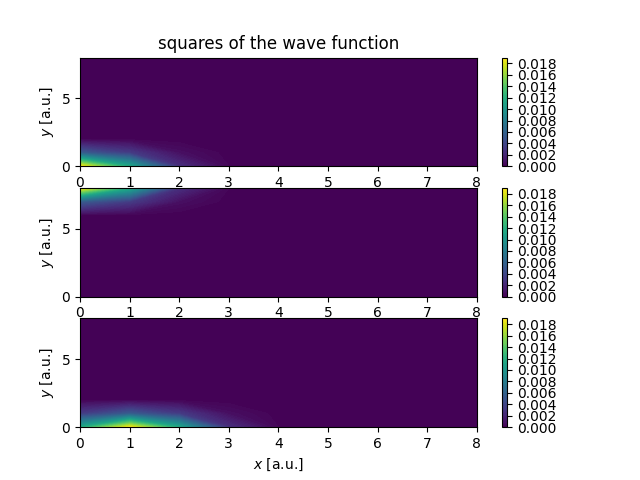
\includegraphics[width=0.75\linewidth]{density_ex1.png}
    \caption{Funkcje bazowe dla \texttt{k = 0, 8, 9}}
    \label{fig:density ex1}
\end{figure}
\subsection{Część 2: Rowiązywanie problemu własnego}
Hamiltonian został wyznaczony analitycznie za pomocą wzorów na całki przekrywania. 
Problem własny rozwiązano numerycznie za pomocą biblioteki \texttt{scipy}. 
Parametry \texttt{omega\_x, omega\_y}, które charakteryzują potencjał kroki kwantowej w dwóch wymiarach na ten moment był dowolnie.
Wyniki przedstawiono na rysunku~\ref{fig:energy of dx ex2}.
\\
\begin{figure}[htp!]
    \centering
    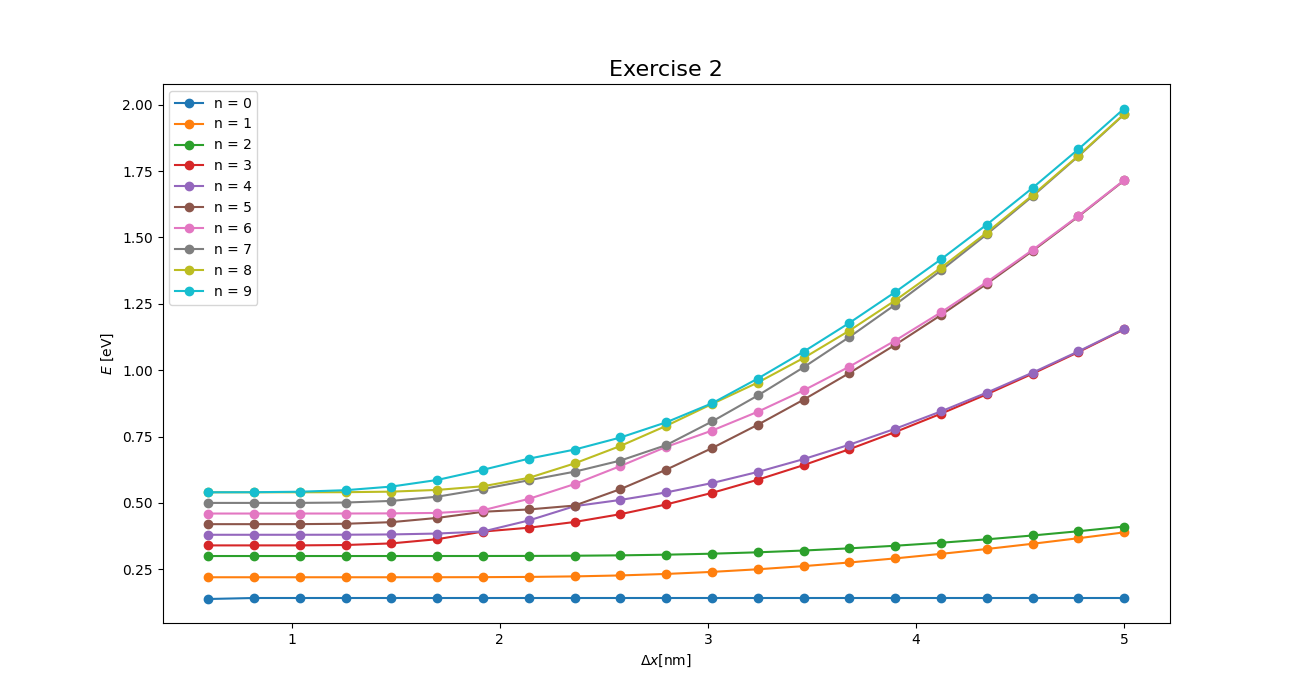
\includegraphics[width=0.75\linewidth]{exercise2.png}
    \caption{Zależność energii kolejnych sanów wzbudzonych dla różnych wartości \texttt{dx}}
    \label{fig:energy of dx ex2}
\end{figure}
\\
Wyraźnie widać tu, że energia dla kolejnych stanów wzbudzonych jest wyższa od poprzedniego.
Zwiększanie \texttt{dx} powodało, że różnice między energiami kolejnych stanów była coraz większa.
\subsection{Część 3: Rozkłady prawdopodobieństwa}
Kolejna część obejmowała przedstawienie rozkładu prawdopodobieństwa dla wyznaczonej funkcji falowej najniższych stanów.
Przy stałych wartościach \texttt{omega\_x = 0.08 / Energy\_hartree, omega\_y = 0.2 / Energy\_hartree} wyplotowane zostały mapy ukazane na rysunku~\ref{fig:energy of dx ex2}.
\begin{figure}[htp!]
    \centering
    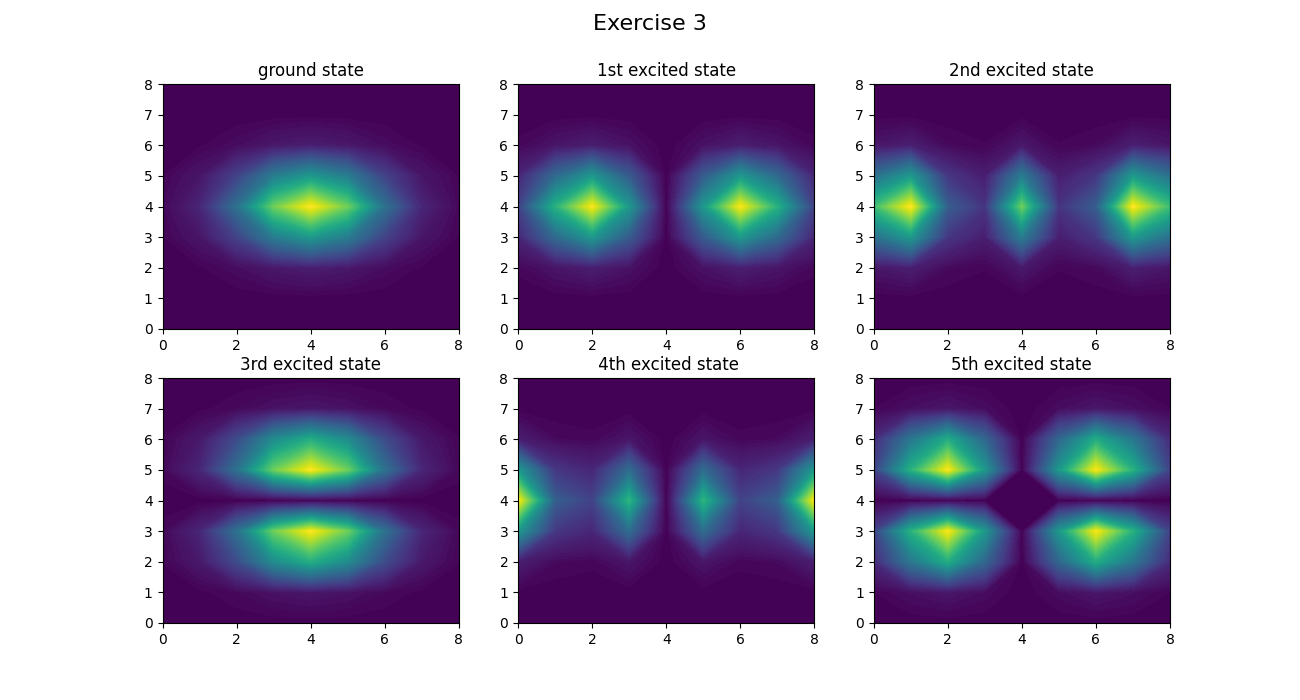
\includegraphics[width=0.75\linewidth]{exercise3.png}
    \caption{Kolejne stany własne kropki w bazie gaussowskiej przy stałych wartościach \texttt{omega\_x, omega\_y}}
    \label{fig:states ex3}
\end{figure}
Zauważmy, że pierwsze trzy stany są wzbudzone oraz piąty tylko w kierunku \texttt{x}, a 4 i~6 - wykazują również w kierunku \texttt{y}.

\subsection{Część 4: Energia}
Kolejnym punktem było wyznaczenie zależności energii od \texttt{hbar * omega\_x} przy stałej wartości \texttt{omega\_y = 200}.
Dodatkowo, wyniki dla kolejnych stanów można było porównać z teoretycznymi wynikami wynikającymi z energii własnych uzyskanych z równania Schr{\"o}dingera dla potencjału oscylatora harmonicznego
\begin{equation}
    E_n = \left(n+\frac{1}{2}\right)\hbar\omega.
    \label{eq: energy disperssion}
\end{equation}
Wyniki oraz porównanie zostało przedstawione na rysunku~\ref{fig:energy of omega ex4}.
\begin{figure}[htp!]
    \centering
    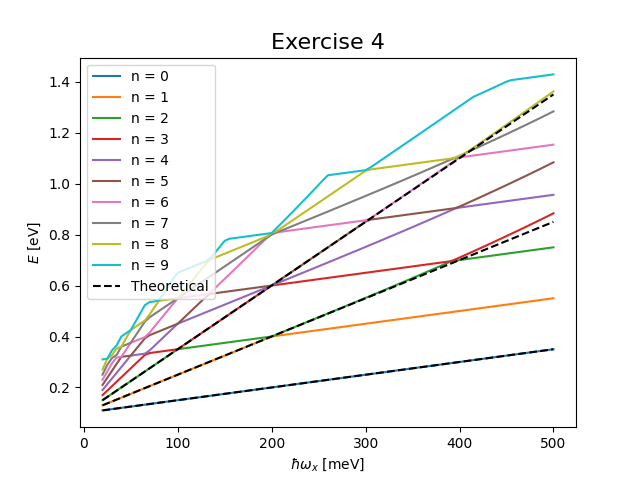
\includegraphics[width=0.75\linewidth]{exercise4.png}
    \caption{Porównanie zależności energii $E$ od $\hbar\omega_x$ przy stałej wartości $\omega_y$.
    Porównanie dotyczy kolejnych stanów wzbudzonych uzyskanych numerycznie oraz wartości teoretycznej podanej wzorem~\eqref{eq: energy disperssion}}
    \label{fig:energy of omega ex4}
\end{figure}
Dla oscylatora harmonicznego oczekujemy liniowej zależności energii od $\omega$. 
Wyniki numeryczne pokazują, że dla niższych stanów taka zależność jest zachowana, ale dla wyższych stanów pojawiają się odchylenia, co może wynikać z efektów numerycznych lub przybliżenia bazowego.
\newpage
\subsection{Część 5: Porównanie z eksperymentem}
Ostatnia część polegała na odpowiednim dobraniu parametru \texttt{omega\_y} tak, aby zgadzały się z wynikami eksperymentalnymi~\cite{Teichmann2013}.
Głównym kryterium było dobranie go tak, aby wzbudzenia występowały jedynie w \texttt{x}.
Przyjęto wartość \texttt{omega\_y = 0.5 / Energy\_hartree}, a rozkłady zostały przedstawione na rysunku~\ref{fig:states ex5}.
\begin{figure}[htp!]
    \centering
    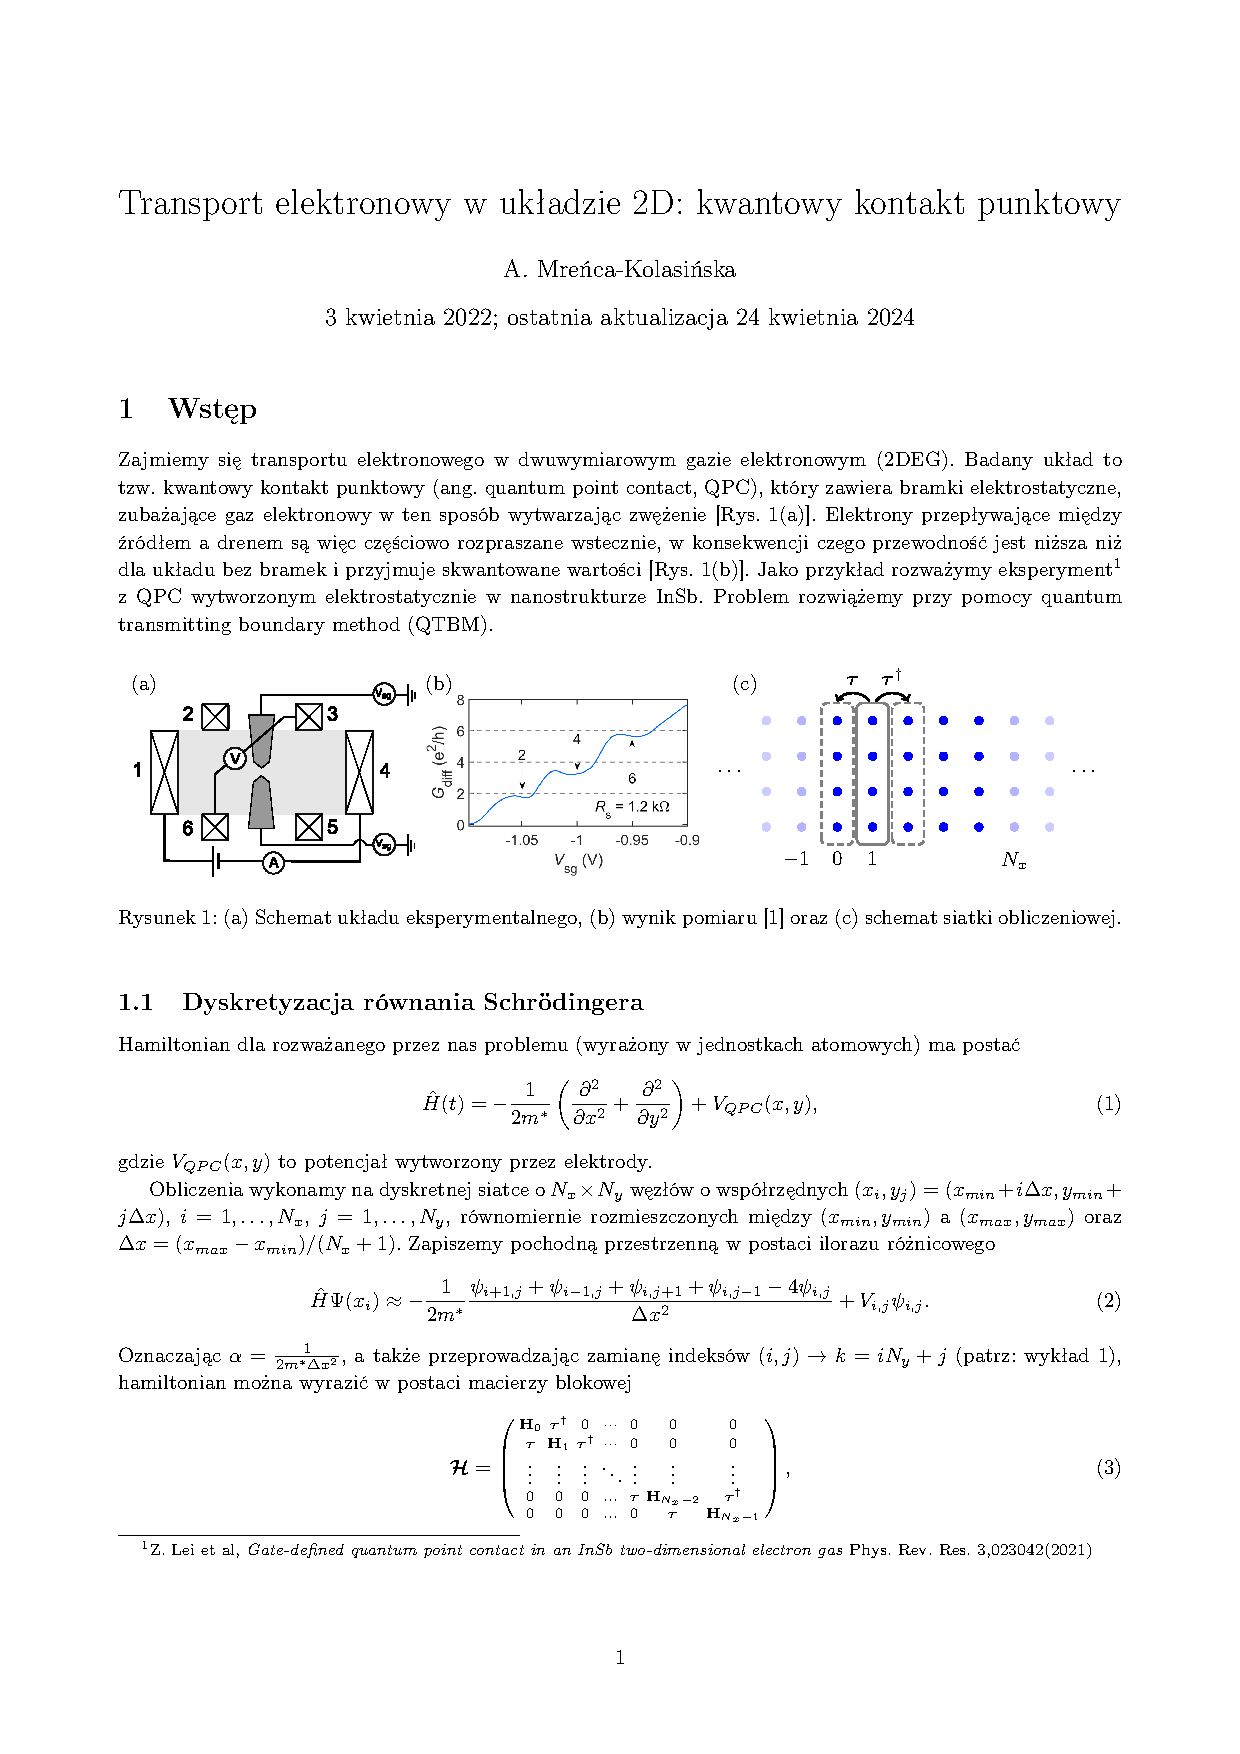
\includegraphics[width=0.75\linewidth]{ex5.png}
    \caption{Kolejne stany kropki kwantowej przy \texttt{omega\_y = (0.5 / Energy\_hartree)} dobranym tak, aby wzbudzenia występowały tylko dla osi \texttt{x}. 
    Wartość \texttt{omega\_x = (0.08 / Energy\_hartree)} jest stała}
    \label{fig:states ex5}
\end{figure}
Jak wpomniano, wzbudzenia występują dla tych parametrów jedynie w kierunku \texttt{x}.

\section{Podsumowanie}
Ćwiczenie polegało na symulacji jednoelektronowej kropki kwantowej w dwóch wymiarach za pomocą metody Galerkina.
Analizowane były charakterystyki systemu, w tym funkcje bazowe metody, rozkłady prawdopodobieństwa kolejnych stanów, wzbudzenia w kierunkach \texttt{x} i \texttt{y} oraz zależność energii od \texttt{omega\_x} - parametru charakteryzującego potencjał kropki w odpowiednim kierunku.
\bibliographystyle{unsrt}
\bibliography{bib}

\end{document}
